\documentclass[a4paper]{article}
\usepackage[english]{babel}
\usepackage[utf8]{inputenc}
\usepackage{algorithm}
%\usepackage{algorithmicx}
\usepackage[noend]{algpseudocode}
\usepackage{amsmath}
\usepackage{graphicx}
\usepackage[colorinlistoftodos]{todonotes}
\usepackage[colorlinks,linkcolor=blue]{hyperref}
\usepackage{color}
%\usepackage[super,square]{natbib}

\renewcommand{\algorithmicrequire}{\textbf{Input:}}
\renewcommand{\algorithmicensure}{\textbf{Output:}}

\title{A prototype of feature-based \emph{Kmeans}}

\author{Changfeng Liu}

\date{\today}

\begin{document}
\maketitle

\begin{abstract}
In this report, I propose a new method to extract features from time series for clustering. In this feature space, the six classes of Synthetic Control\cite{dataset} data set are located separately. With \emph{Kmeans}, it can mostly distinguish the six classes. I introduce the design of feature vector, the experiment results and some potential future work in this report.
\end{abstract}

\setcounter{tocdepth}{2}
\tableofcontents

\newpage
\section{Introduction}
Generally, there are three kinds of time series clustering: raw-data-based, feature-based and model-based\cite{survey}. In this report, I use feature-based \emph{K-means} to cluster time series. 

The basic idea is to extract several features which are able to distinguish time series with different frequent patterns. In other words, in this feature space, time series with different patterns are far from each other while time series with similar patterns are close.

I implemented this algorithm and tried it on ``Synthetic Control Chart Time Series''\cite{dataset} data set.

\section{Feature Vector Design}
I designed a three-dimension feature vector in this very first version, namely for seasonality, global trend and shift detection.

\subsection{D1: Seasonality}
\subsubsection{Basic Idea}
Seasonal (cyclic) time series have obvious periodic components and thus in frequent spectrum they should have larger amplitudes.

The aim of seasonality dimension is to distinguish seasonal time series (no matter how long period they have) from non-seasonal time series.
\subsubsection{Implementation}
Algorithm \ref{alg:season} shows the details of how to obtain the values of seasonality.

\begin{algorithm}
\caption{Seasonality Dimension} \label{alg:season}
\begin{algorithmic}[1] 
\Require{$ts$}\Comment{Raw time series data.}
\Ensure{$seasonality$}
	\State $ts\_norm \gets$ \Call{Normalize}{$ts$}
	\State $spectrum \gets$ \Call{FFT}{$ts\_norm$}
	\State $amplitude \gets$ \Call{Abs}{$spectrum$}
	\State $tmp \gets$ \Call{Max}{$ amplitude(3:length-2) $}\Comment{Discard the first two points and the last two points.}
	\State $seasonality \gets$ \Call{Signal}{$tmp$} * (\Call{Abs}{$tmp$})$^{0.5}$
	\State
	\Function {Normalize}{$ts$}
		\State $average \gets$ \Call{Mean}{$ts$}
		\State $std \gets$ \Call{StandardDeviation}{$ts$}
		\State $ts\_norm \gets (ts - mean) / std$
		\State \Return{$ts\_norm$}
	\EndFunction
\end{algorithmic}
\end{algorithm}

Because $ts\_norm$ is a real number sequence, $spectrum$ is symmetric. The first and last points of $amplitude$ are direct current components, which are zero after normalization, thus I discard them. 

I also discard the second and penultimate points because the values of them can be large in some non-seasonal time series. This is totally empirical and I haven't figured out the reason.

\subsubsection{Results}
Figure \ref{fig:seasonality} is a histogram. The X axis shows the value of this feature, and the Y axis shows the numbers of time series whose values of this feature are in a specific X-value interval.

From figure \ref{fig:seasonality}, we can easily see that cyclic time series are separated from other five kinds of time series.

\begin{figure}[htbp]
\centering
\includegraphics[width=1\textwidth]{seasonality.png}
\caption{\label{fig:seasonality}Seasonality histograms of six kinds of time series.}
\end{figure}

\subsection{D2: Global Trend}
Global trend is to show how much the value increases or decreases by from the start to the end. 

\subsubsection{Basic Idea}
Apply normalization and smoothing firstly in order to avoid scaling and noise, and then calculate the difference between last point and first point.

\subsubsection{Implementation}
Algorithm \ref{alg:gt} shows the details.

\begin{algorithm}
\caption{Global Trend Dimension} \label{alg:gt}
\begin{algorithmic}[1] 
\Require{$ts$}\Comment{Raw time series data.}
\Ensure{$global\_trend$}
	\State $ts\_norm \gets$ \Call{Normalize}{$ts$}
	\State $ts\_smooth \gets$ \Call{Smoothing}{$ts\_norm, 6$}
	\State $global\_trend \gets ts\_smooth(length) - ts\_smooth(1)$
	\State
	\Function {Normalize}{$ts$}
		\State $average \gets$ \Call{Mean}{$ts$}
		\State $std \gets$ \Call{StandardDeviation}{$ts$}
		\State $ts\_norm \gets (ts - mean) / std$
		\State \Return{$ts\_norm$}
	\EndFunction
	\State
	\Function {Smoothing}{$ts, wl$}\Comment{$wl$ is the window length}
		\State $window \gets [1/(2*wl);$ \Call{Ones}{$wl-1,1$}$*(1/wl); 1/(2*wl)]$
		\State $ts\_smooth \gets$ \Call{Convolution}{$ts\_norm, window$}
		\State \Return{$ts\_smooth$}
	\EndFunction
	%\State
	%\Function {GetSlope}{$ts$}
	%	\For {$ i = 1 \to length - 1$} 
	%		\State $slope(i) \gets ts(i+1) - ts(i)$
	%	\EndFor
	%	\State \Return{$slope$}
	%\EndFunction
\end{algorithmic}
\end{algorithm}

\subsubsection{Results}
The results are shown is Figure \ref{fig:gt}. As you can see, it can easily divide the six classes into three groups: (increasing trend, up shift), (decreasing trend, down shift) and (normal, cyclic). However it is hard for global trend to tell the differences within a group, for example, increasing trend and up shift.

\begin{figure}[htbp]
\centering
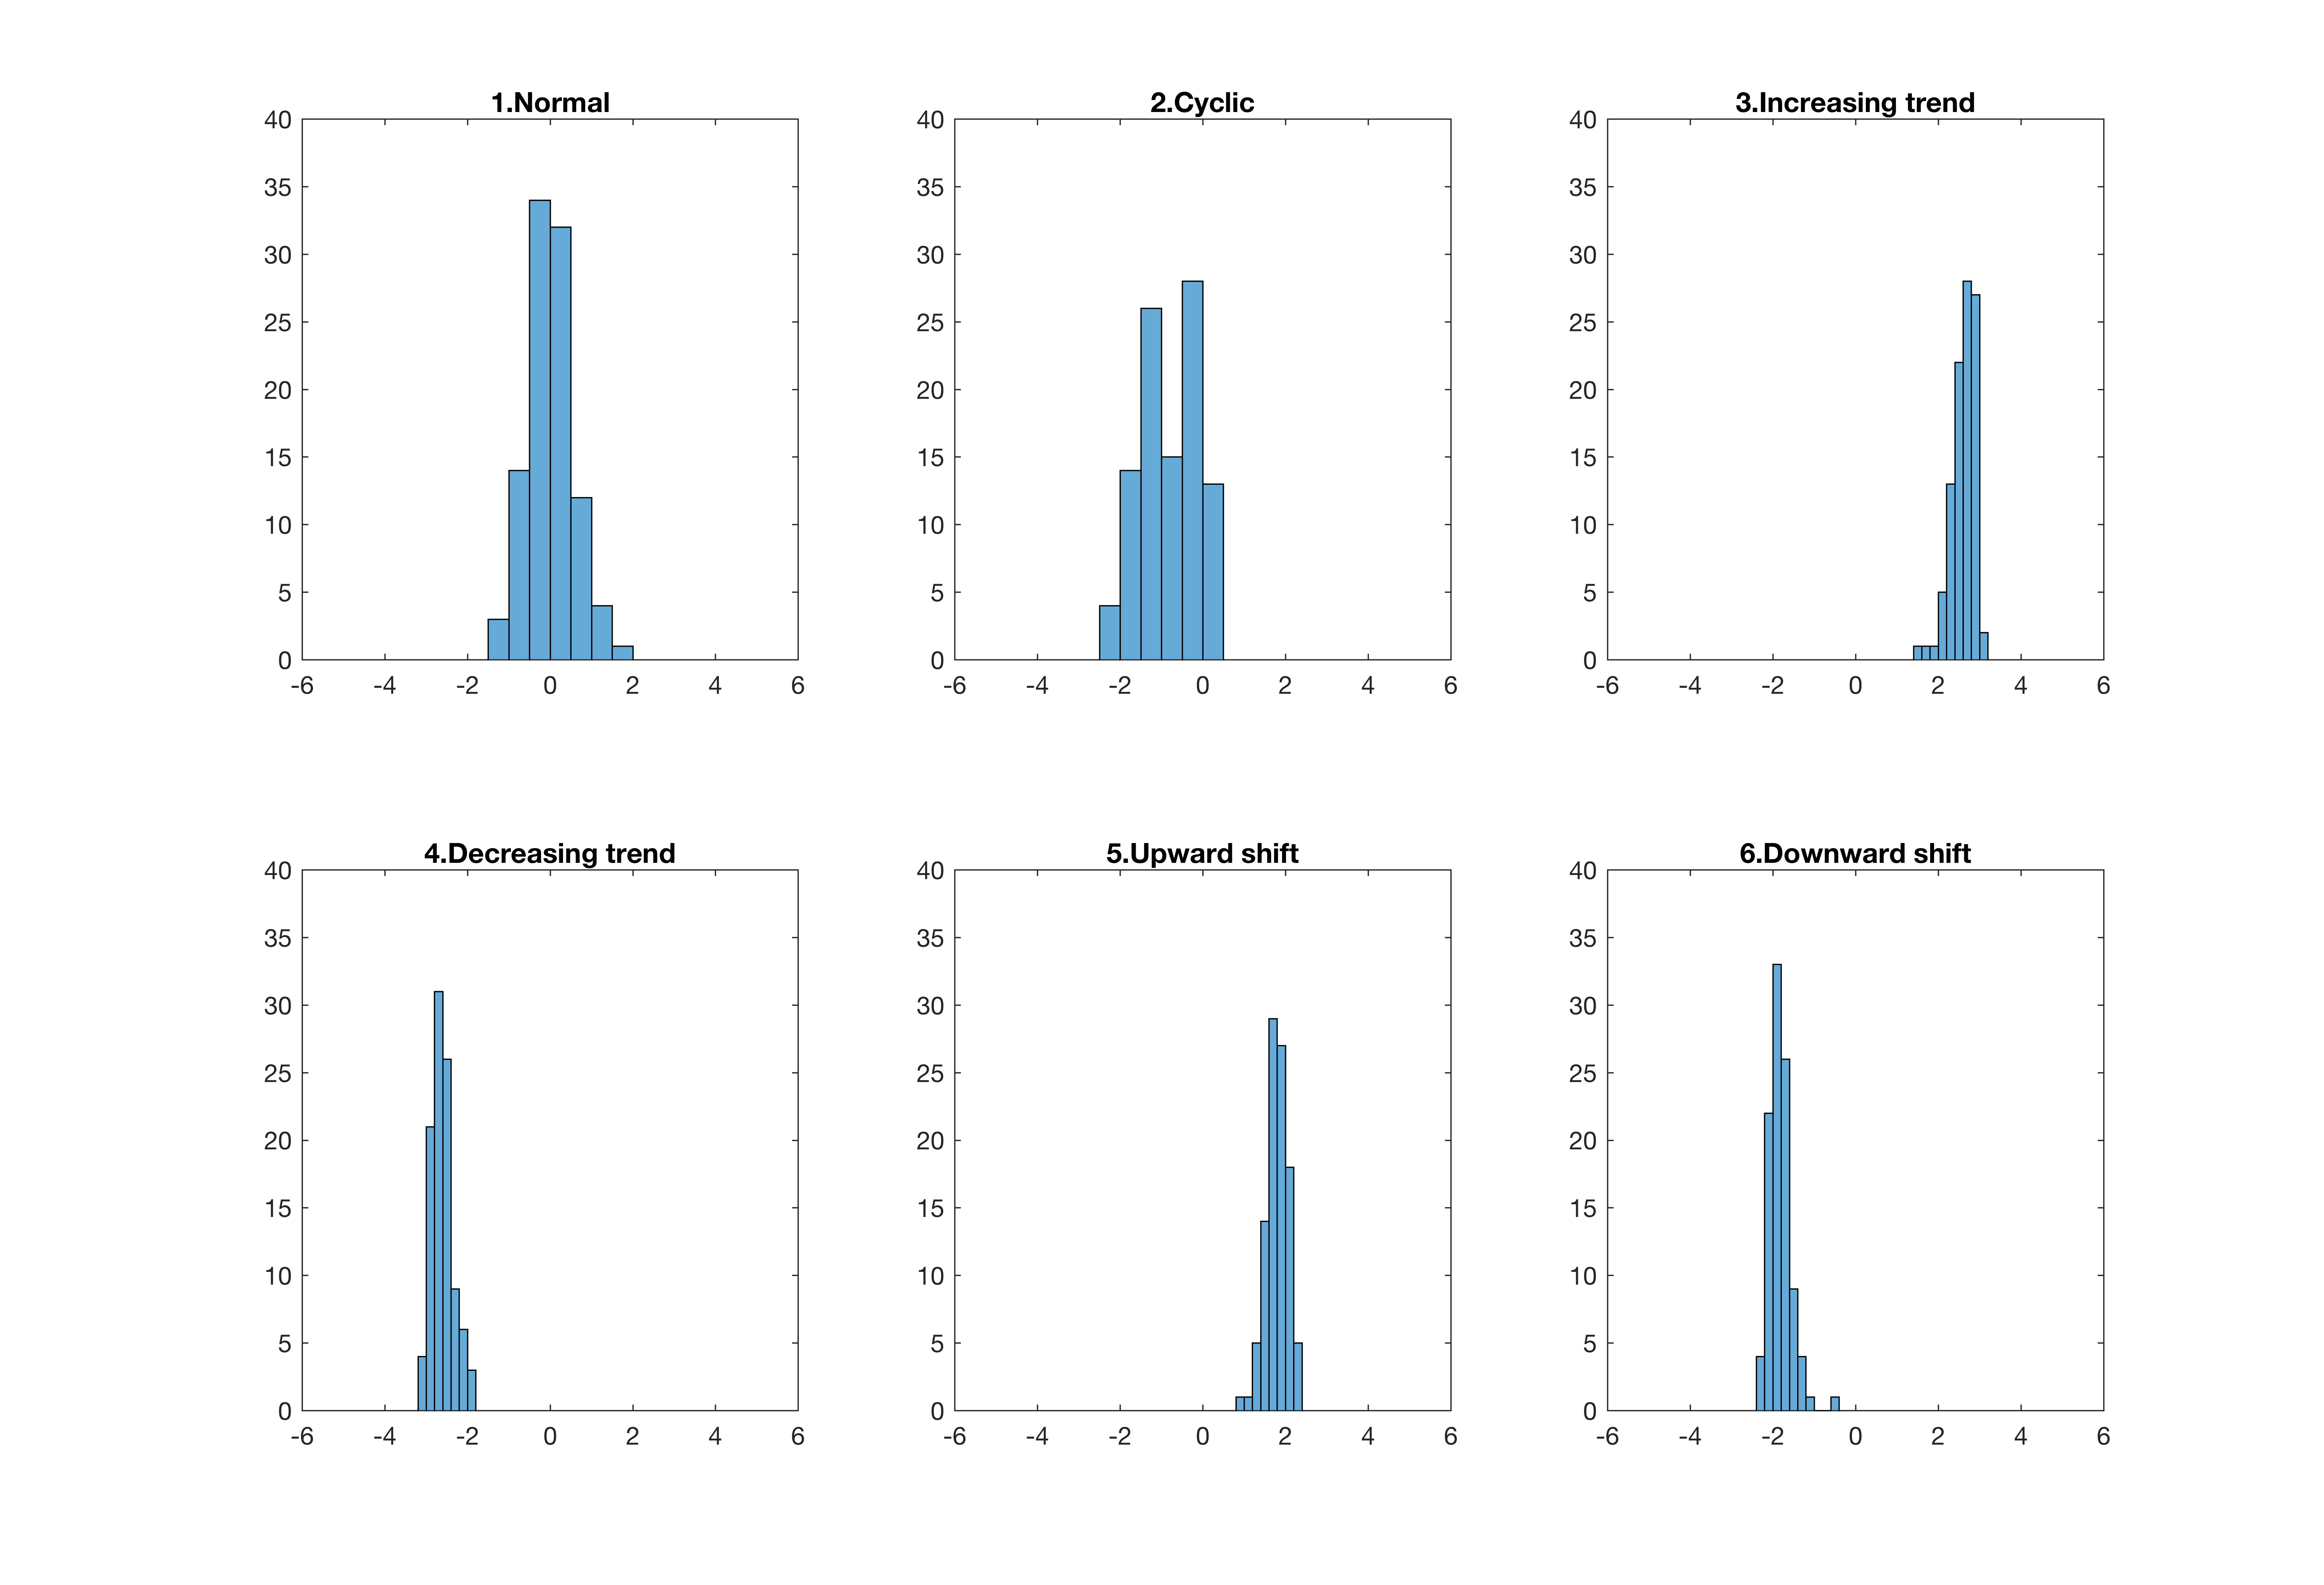
\includegraphics[width=0.9\textwidth]{gt.png}
\caption{\label{fig:gt}Global trend histograms of six kinds of time series.}
\end{figure}

\subsection{D3: Up/Down Shifts vs Increasing/Decreasing Trend}
Since we have been able to distinguish cyclic, up trend and down trend with the help of D1 and D2, what we need to do is to tell the differences between shifts and steady trends.
\subsubsection{Basic Idea}
The basic idea is to detect the shifts of time series and leverage that up/down shifts contribute most of the total increasement / decreasement.

\subsubsection{Implementation}
Algorithms \ref{alg:shift} shows the details.

\begin{algorithm}
\caption{Shift Dimension} \label{alg:shift}
\begin{algorithmic}[1] 
\Require{$ts$}\Comment{Raw time series data.}
\Ensure{$shift$}

	\State $ts\_norm \gets$ \Call{Normalize}{$ts$}
	\State $ts\_smooth \gets$ \Call{Smoothing}{$ts\_norm, 6$}
	\State $slope\_step \gets$ \Call{GetStepSlope}{$ts\_smooth$}
	\State $global\_trend \gets ts\_smooth(length) - ts\_smooth(1)$
	\State $slope\_step\_abs \gets$ \Call{Abs}{$slope\_step$}
	\State $shift \gets global\_trend /$ \Call{Max}{ $slope\_step\_abs$}
	\State
	\Function {Normalize}{$ts$}
		\State $average \gets mean(ts)$
		\State $std \gets standard\_deviation(ts)$
		\State $ts\_norm \gets (ts - mean) / std$
		\State \Return{$ts\_norm$}
	\EndFunction
	\State
	\Function {Smoothing}{$ts, wl$}\Comment{$wl$ is the window length}
		\State $window \gets [1/(2*wl);$ \Call{Ones}{$wl-1,1$}$*(1/wl); 1/(2*wl)]$
		\State $ts\_smooth \gets$ \Call{Convolution}{$ts\_norm, window$}
		\State \Return{$ts\_smooth$}
	\EndFunction
	\State
	\Function {GetStepSlope}{$ts, step$}
		\For {$ i = 1 \to length- step$} 
			\State $slope\_step(i) \gets ts(i+step) - ts(i)$
		\EndFor
		\State \Return{$slope\_step$}
	\EndFunction
	
\end{algorithmic}
\end{algorithm}

\subsubsection{Results}
Figure \ref{fig:shift} shows the histograms of shift dimension. We can separate shifts from steady trends using shift dimension.

\begin{figure}[htbp]
\centering
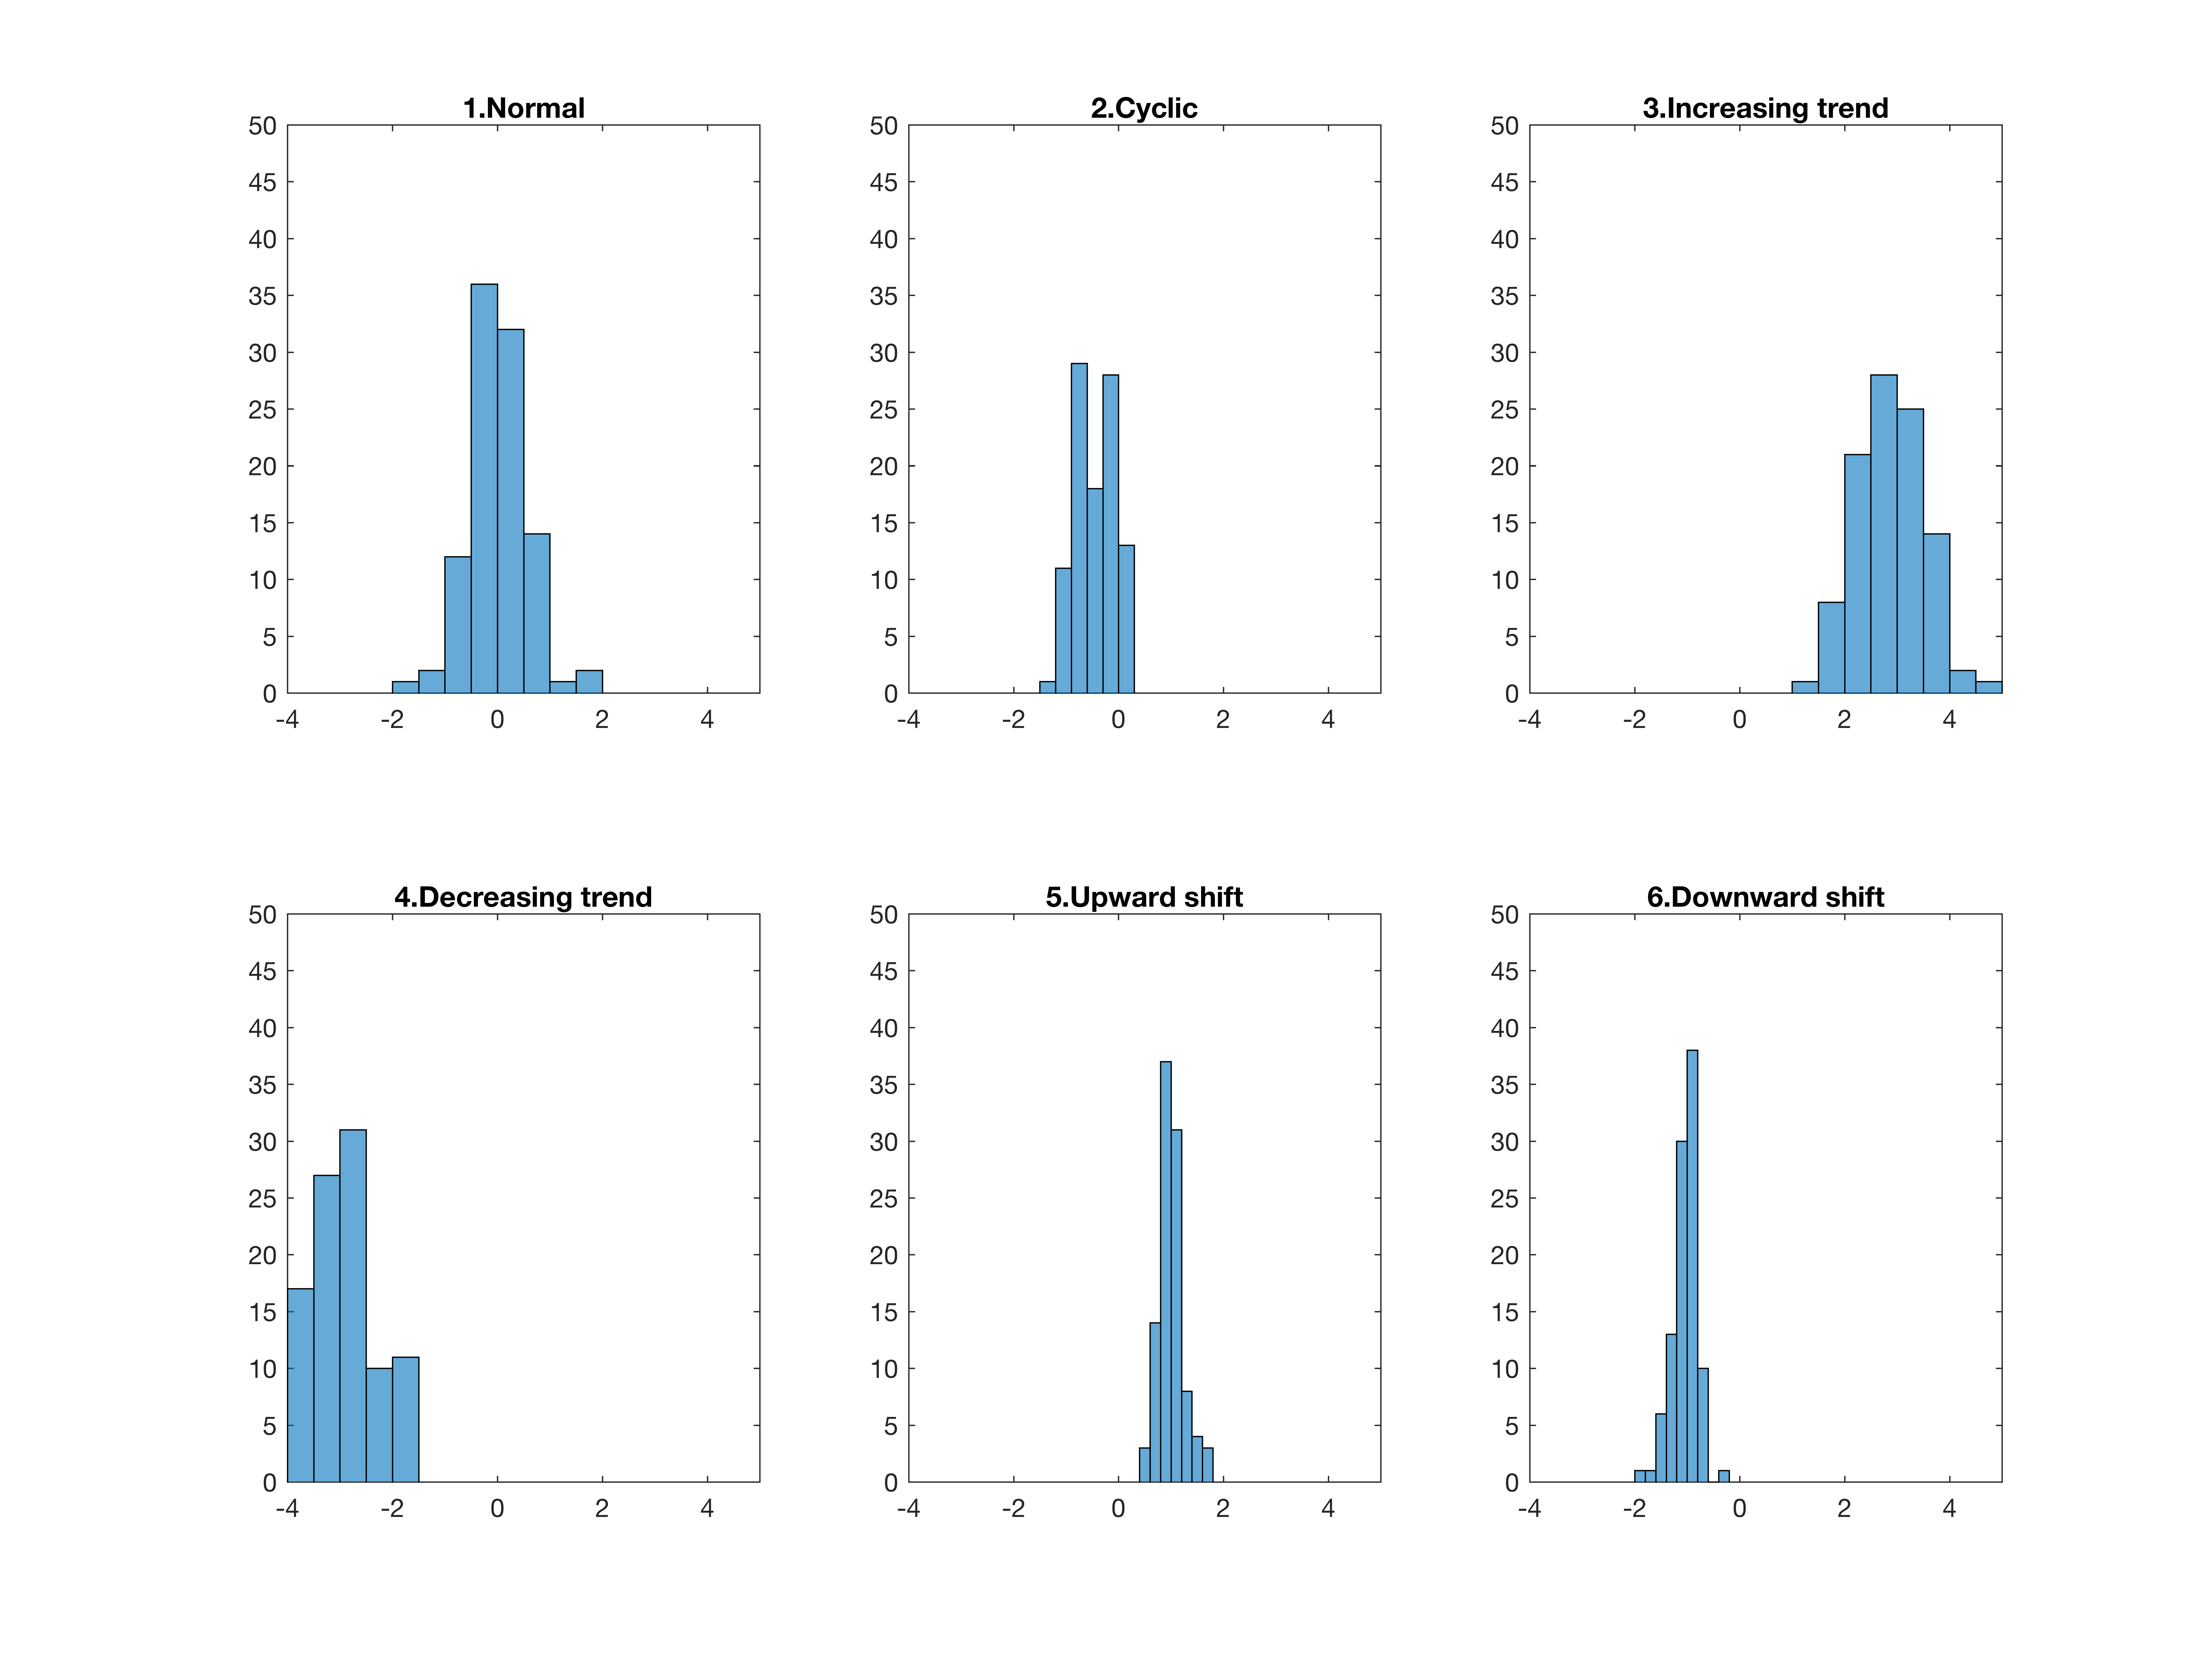
\includegraphics[width=1\textwidth]{shift.png}
\caption{\label{fig:shift}Shift histograms of six kinds of time series.}
\end{figure}

\subsection{Other Processing}
After obtaining all features of time series, I use them to form the feature vectors. Then apply normalization to each dimension for all time series data. The normalization is the same as $Normalize$ function in algorithm \ref{alg:season}.

\section{Experiments}
\subsection{Groundtruth}
The correct clusters in feature space is shown in Figure \ref{fig:groundt}. Six classes of time series are six separated clusters in feature space, which is good for Kmeans method.
\begin{figure}[htbp]
\centering
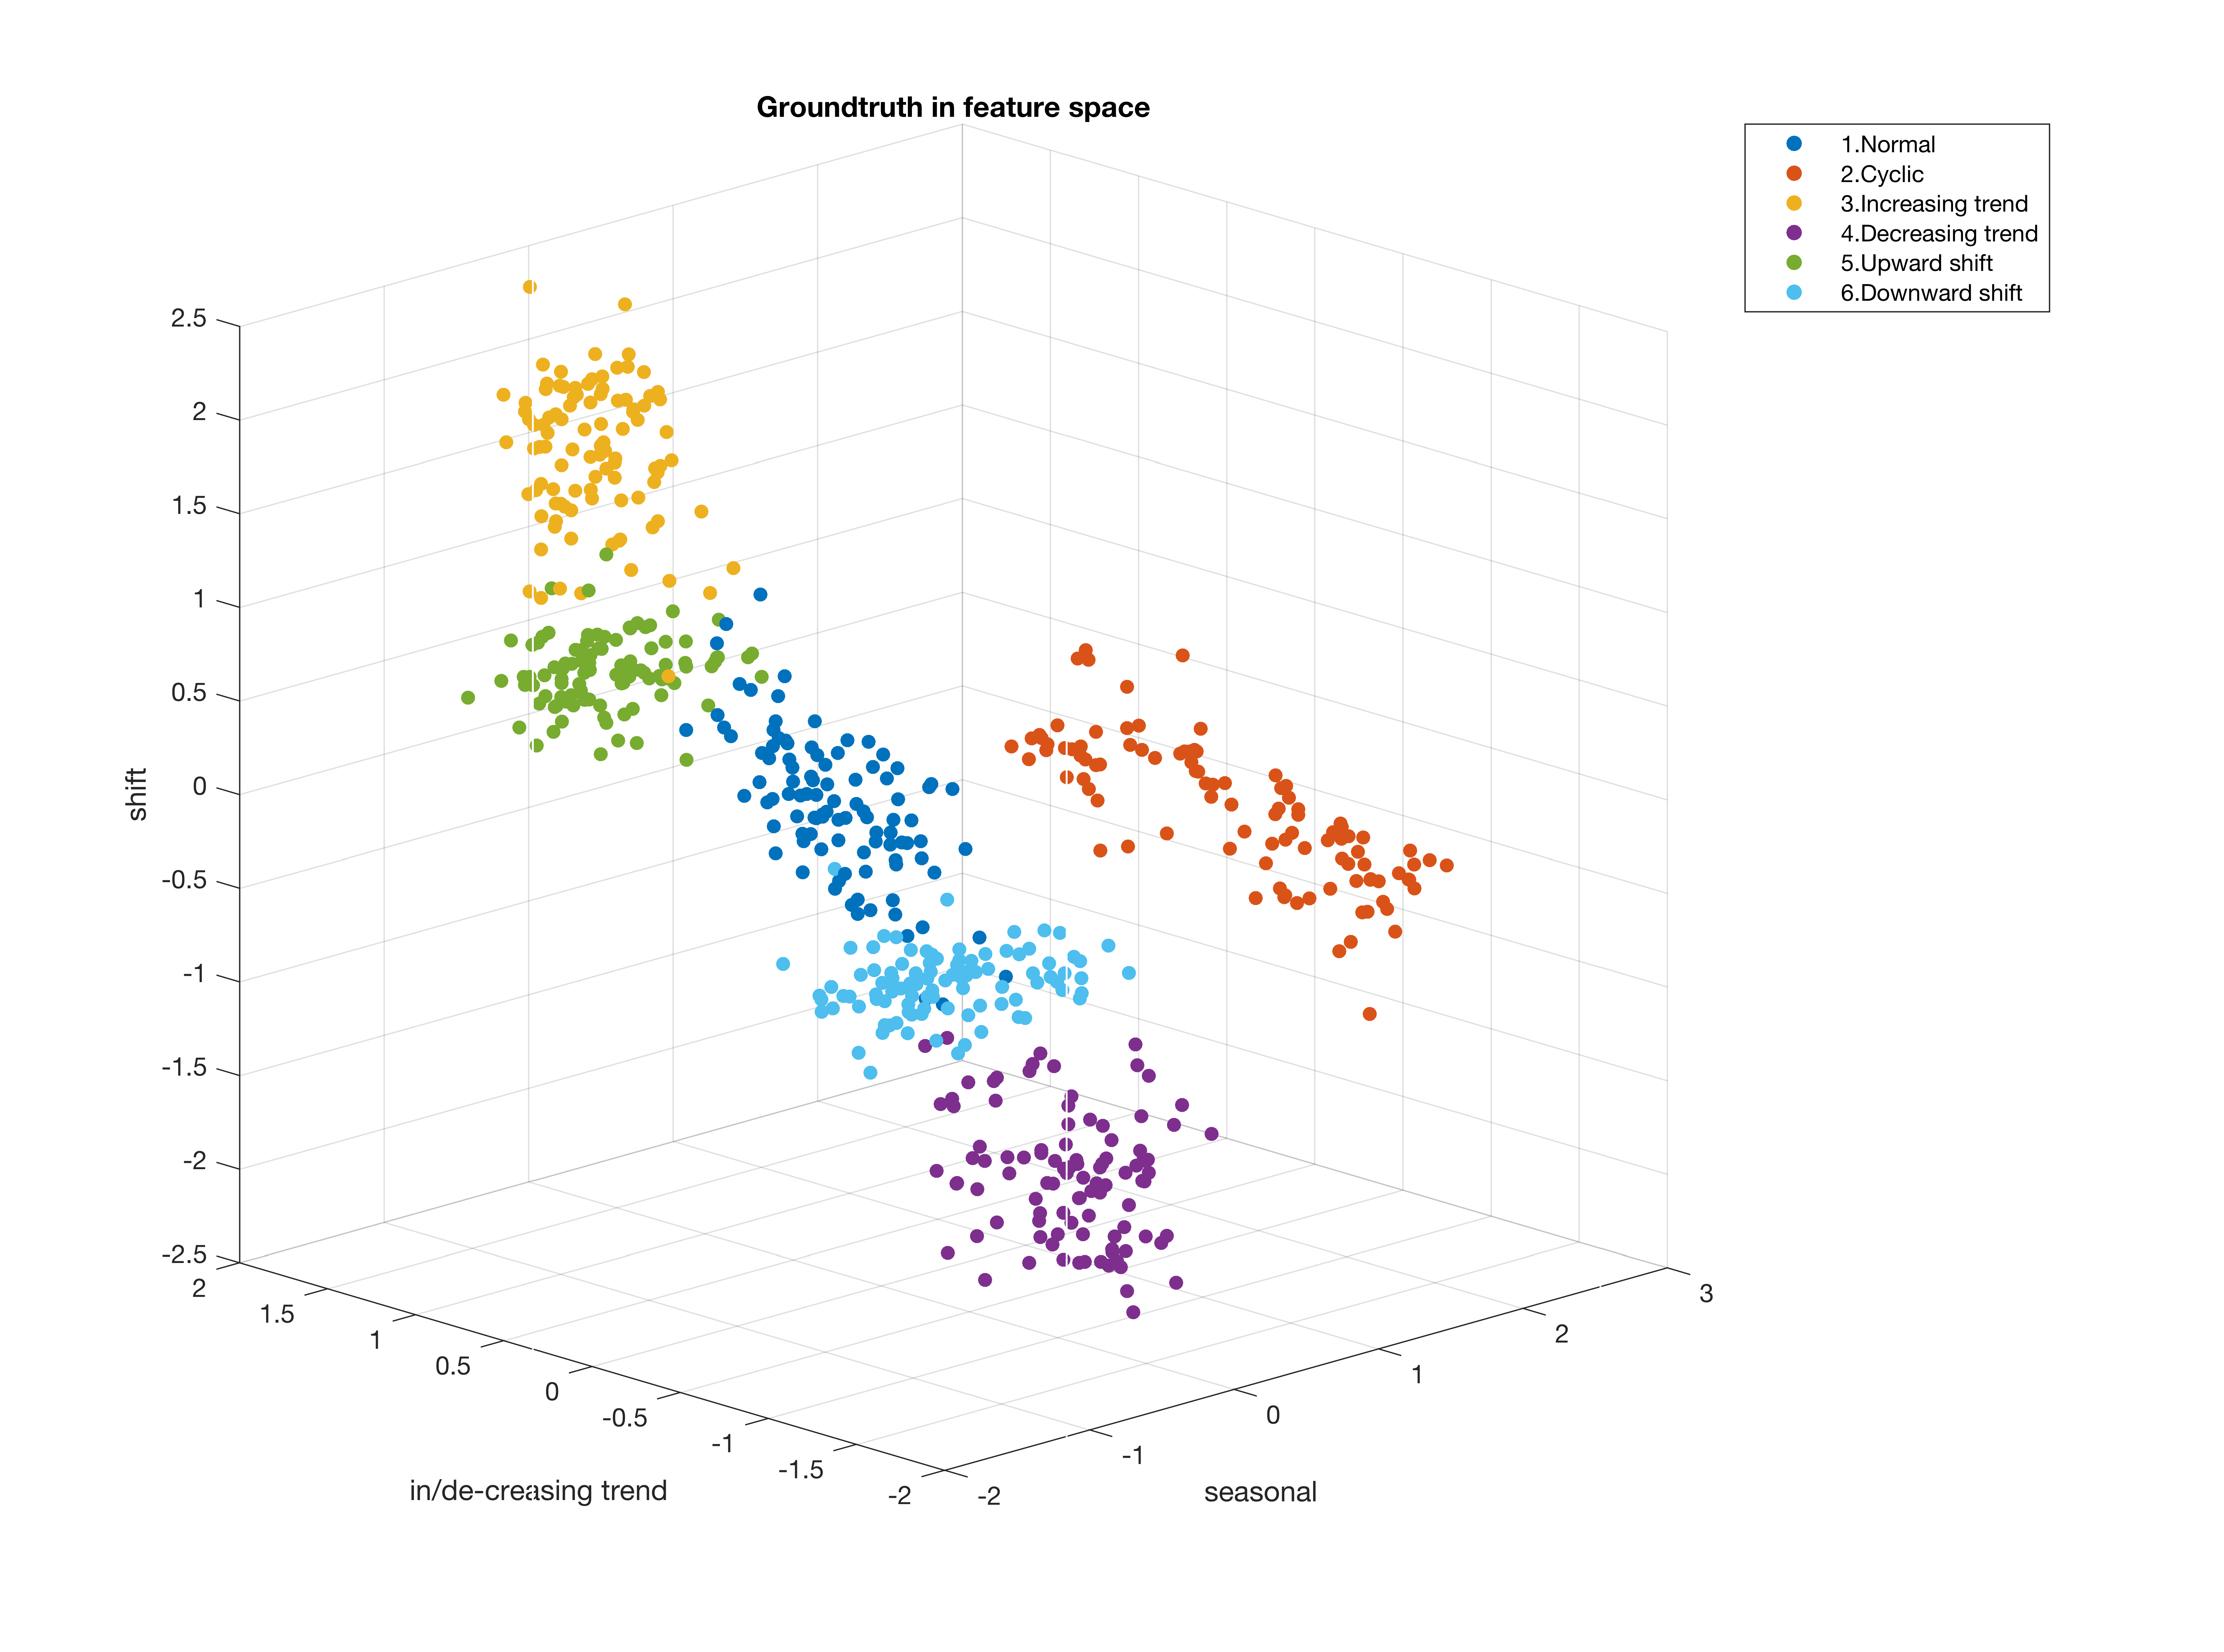
\includegraphics[width=1\textwidth]{groundt.png}
\caption{\label{fig:groundt}Correct clusters in feature space.}
\end{figure}

\subsection{Good Results}
Figure \ref{fig:goodr} shows a good clustering result with 94\% accuracy. Table \ref{tab:good} shows the clustering details where red numbers mean right clusters.

\begin{figure}[htbp]
\centering
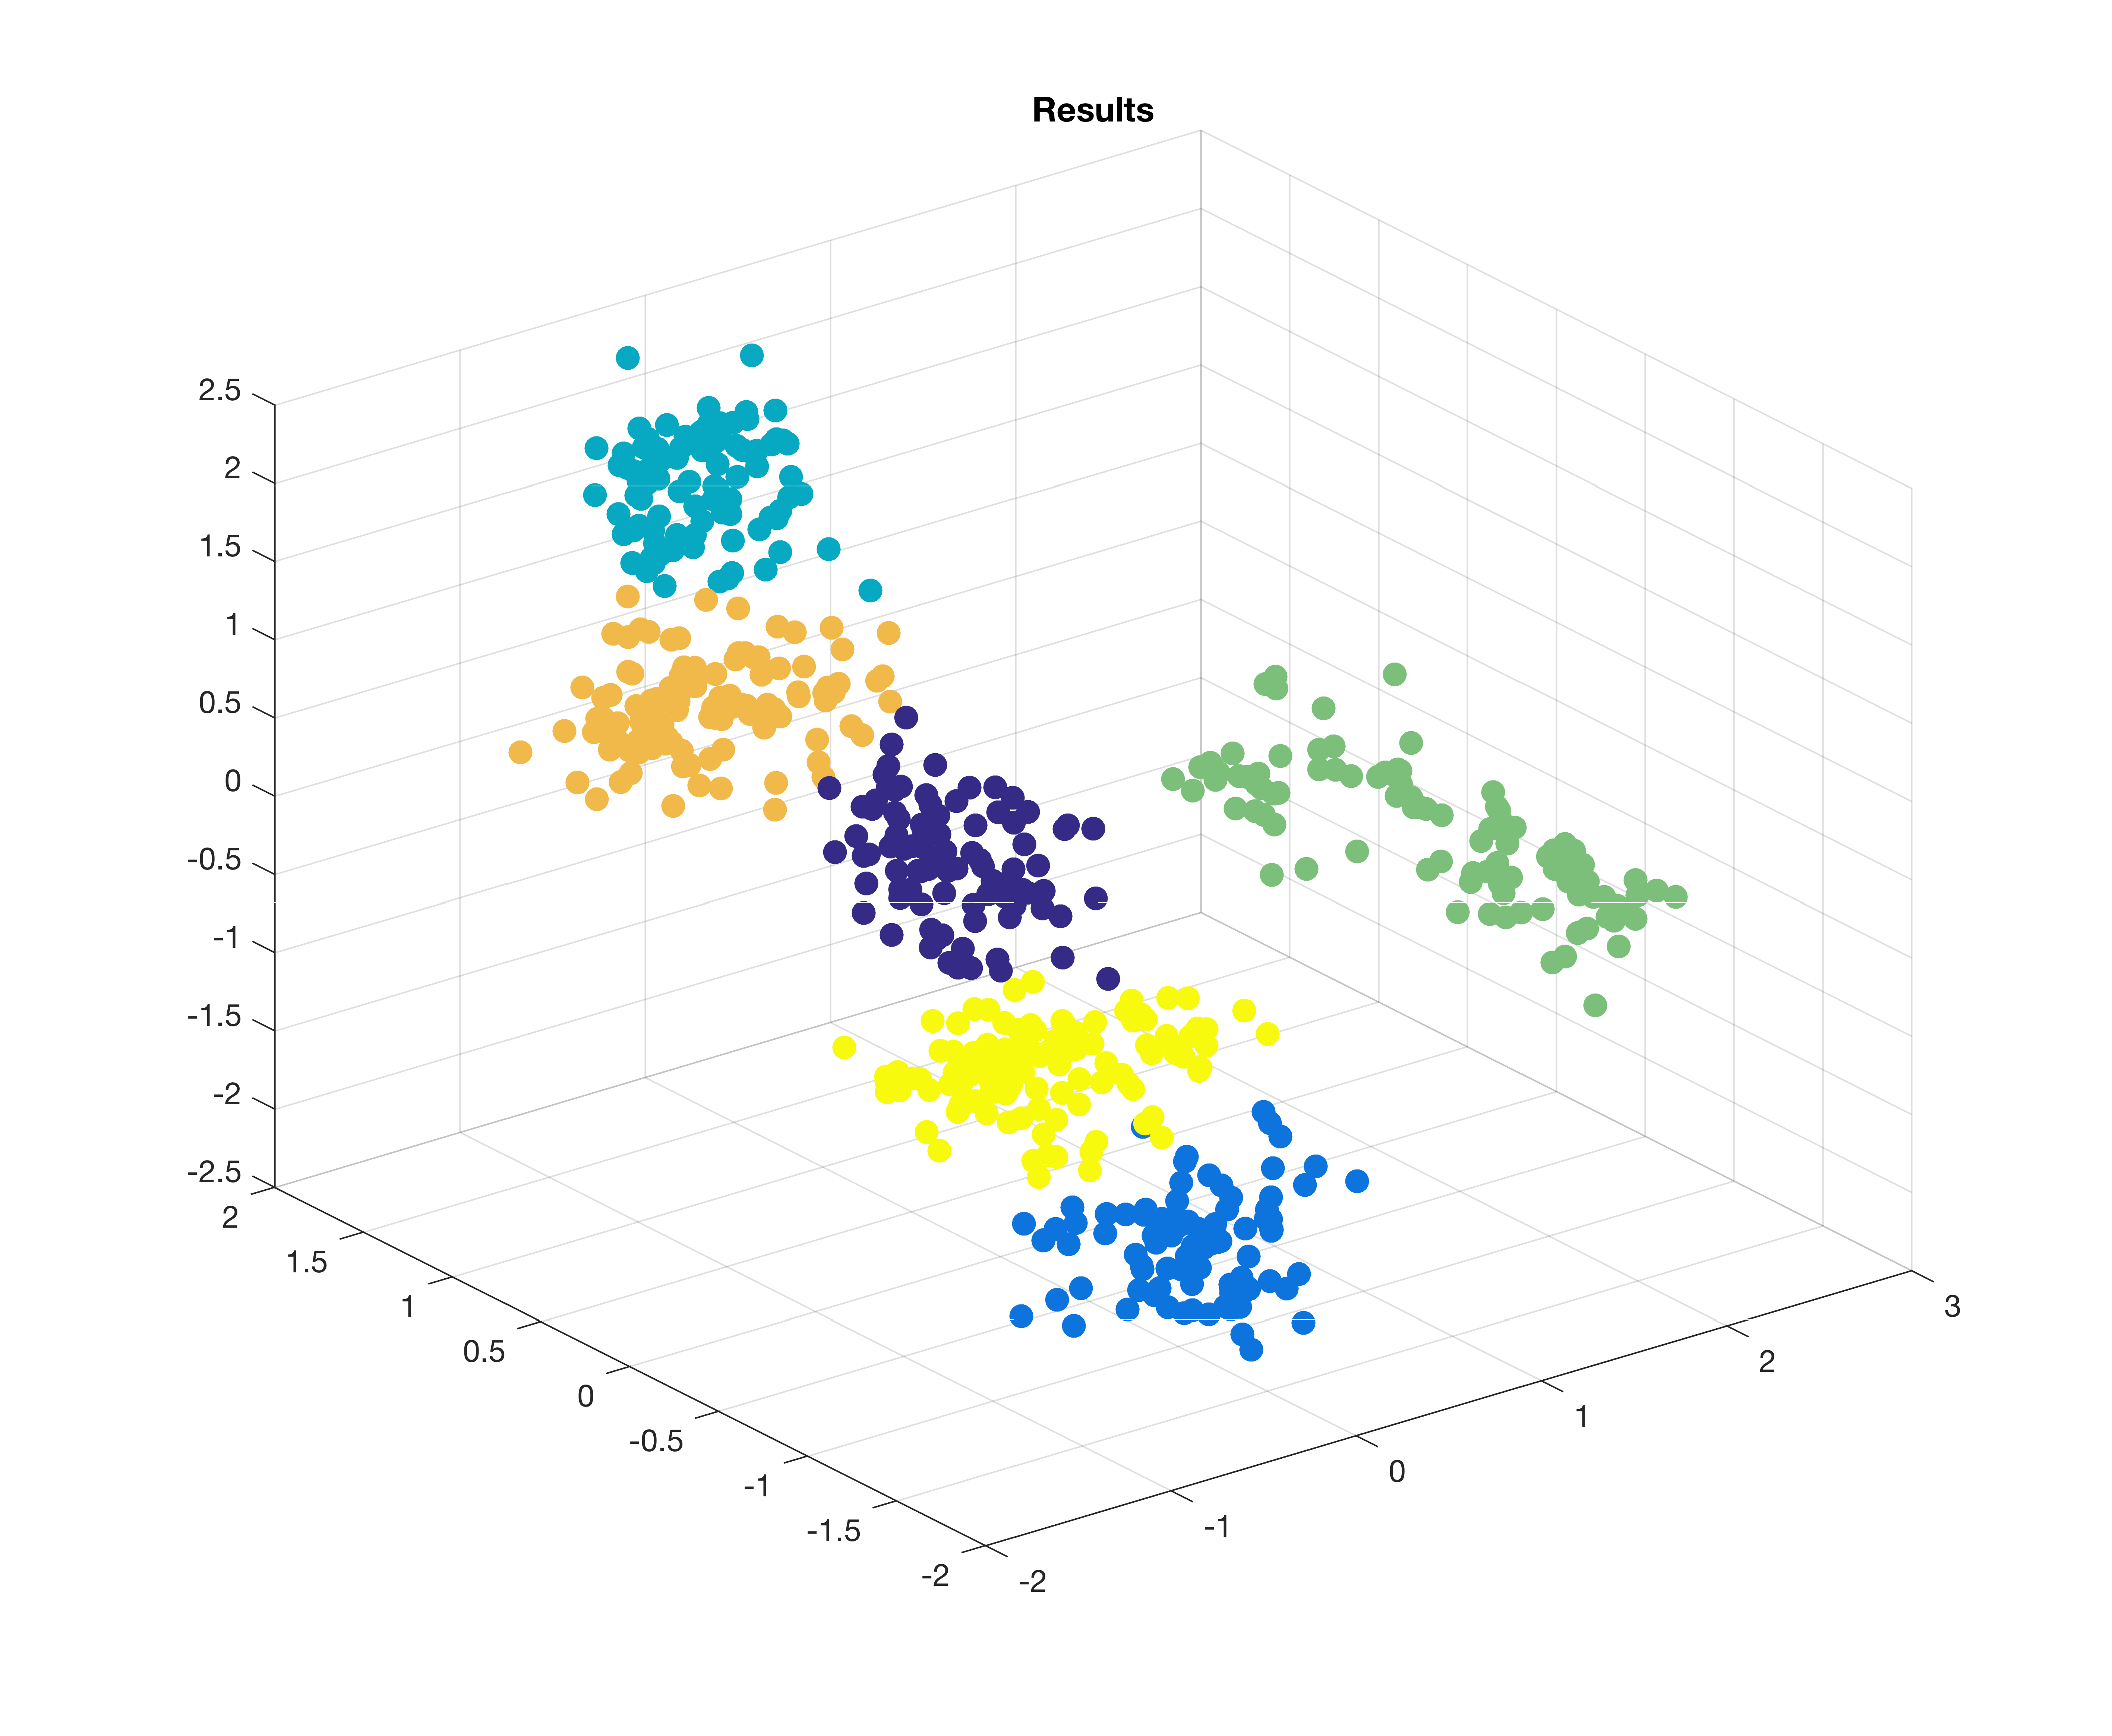
\includegraphics[width=1\textwidth]{goodr.png}
\caption{\label{fig:goodr}Good clustering result using Kmeans.}
\end{figure}

\begin{table}[htbp]
\caption{\label{tab:good}Cross table for a good result and groundtruth.}
\centering
\begin{tabular}{|c|c|c|c|c|c|c|}
 \hline
  & Normal & Cyclic & Increasing& Decreasing & Up shift &Down shift\\
 \hline
Cluster 1 & {\color{red}{87}} & 0 & 0 & 0 & 0 & 2 \\
 \hline
Cluster 2 & 0 & 0 & 0 & {\color{red}{88}} & 0 & 0\\
 \hline
Cluster 3 & 0 & 0 & {\color{red}{91}} & 0 & 0 & 0 \\
 \hline
Cluster 4 & 0 & {\color{red}{100}} & 0 & 0 & 0 & 0\\
 \hline
 Cluster 5 & 8 & 0 & 9 & 0 & {\color{red}{100}} & 0\\
 \hline
 Cluster 6 & 5 & 0 & 0 & 12 & 0 & {\color{red}{98}}\\
 \hline
\end{tabular}
\end{table}

\subsection{Not So Good Results}\label{sec:bad}
Figure \ref{fig:badr} shows a not so good clustering result with 72\% accuracy. Table \ref{tab:bad} shows the clustering details where red numbers indicate right clusters.

\begin{figure}[htbp]
\centering
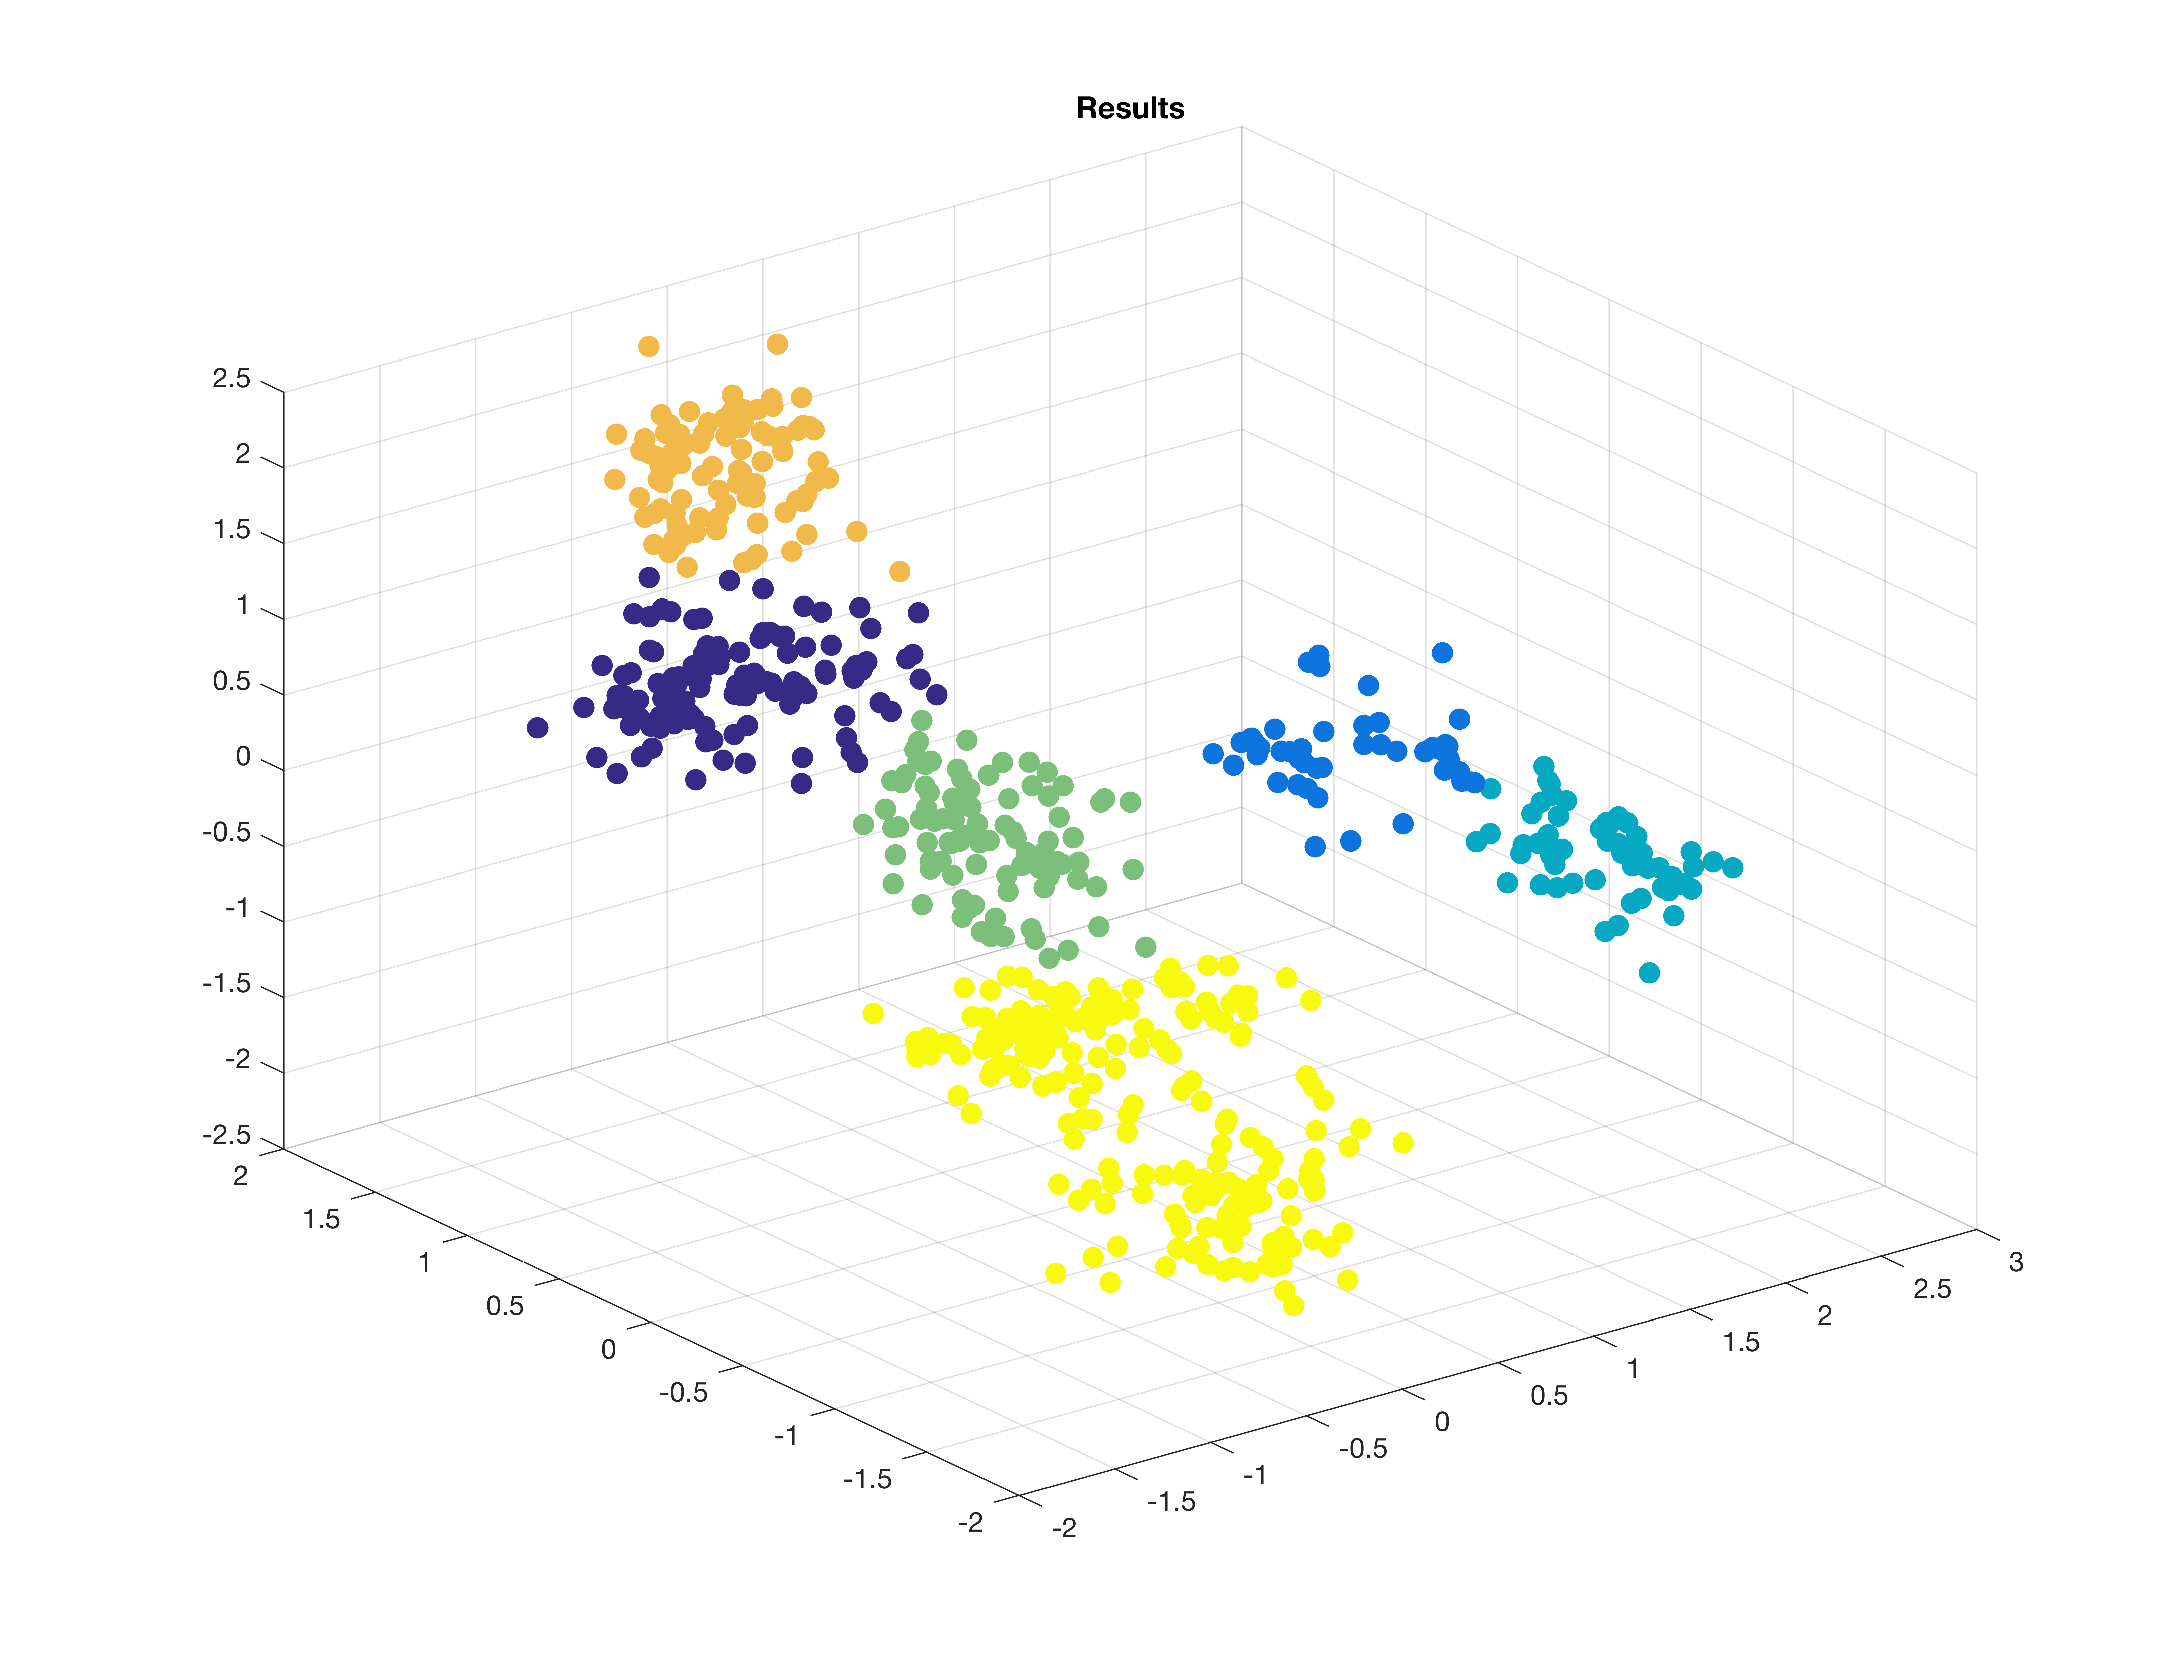
\includegraphics[width=1\textwidth]{badr.png}
\caption{\label{fig:badr}Not so good clustering result using Kmeans.}
\end{figure}

\begin{table}[htbp]
\caption{\label{tab:bad}Cross table for a not so good result and groundtruth.}
\centering
\begin{tabular}{|c|c|c|c|c|c|c|}
 \hline
  & Normal & Cyclic & Increasing& Decreasing & Up shift &Down shift\\
 \hline
Cluster 1 & 10& 0 & 9 & 0 & {\color{red}{100}}  & 0 \\
 \hline
Cluster 2 & 0 &45  & 0 & 0 & 0 & 0\\
 \hline
Cluster 3 & 0 & {\color{red}{55}}  & 0 & 0 & 0 & 0 \\
 \hline
Cluster 4 & {\color{red}{87}}  & 0 & 0 & 0 & 0 & 2\\
 \hline
 Cluster 5 & 0 & 0 & {\color{red}{91}}  & 0 & 0 & 0\\
 \hline
 Cluster 6 & 3 & 0 & 0 & {\color{red}{100}}  & 0 & 98\\
 \hline
\end{tabular}
\end{table}

\section{Potential Work}
\subsection{Decomposition}
We could do \emph{time series decomposition} first and divide a time series sequence into three components: seasonality, trend and noise. Actually, the smoothing operation of current algorithm is a part of decomposition.
\subsection{Representative Trends}
Try to find a proper way to find the representative trend of each cluster. 
\subsection{Other Data Sets}
I will try this algorithm on other data sets and add more features based on visual perception to make this algorithm more robust and universal.
\subsection{Initialization of Kmeans}
There might be some problems with the initialization of Kmeans, which likely leads to the not good result of \ref{sec:bad}. I will try to figure it out.

%%%%%%%%%%%%%%%%%%%%%%%%%%%%%%%%%%%%%%%%%%%%%%
\begin{thebibliography}{99}
\bibitem{survey}
Liao, T. Warren. ``Clustering of time series data—a survey.'' \emph{Pattern recognition} 38.11 (2005): 1857-1874.

\bibitem{dataset}
UCI Machine Learning Repository. ``Synthetic Control Chart Time Series.''\url{http://archive.ics.uci.edu/ml/databases/synthetic_control/synthetic_control.data.html}.

\end{thebibliography}

\end{document}